% ============================================================
% 压轴题模型精讲 — 初中数学培优
% 编译命令：xelatex -interaction=nonstopmode 培优专题4_压轴题模型精讲.tex
% ============================================================
\documentclass[12pt, a4paper]{ctexart}
\usepackage[margin=2.2cm]{geometry}
\usepackage{amsmath, amssymb, amsthm}
\usepackage{enumitem}
\usepackage{tcolorbox}
\usepackage{booktabs}
\usepackage{array}
\usepackage{fancyhdr}
\usepackage{xcolor}
\usepackage{tikz}
\usepackage{hyperref}
\usepackage{graphicx}
\usepackage{multirow}
\usepackage{pgfplots}
\pgfplotsset{compat=1.18}
\usetikzlibrary{angles, quotes, patterns, decorations.markings, calc, positioning}

% 颜色定义
\definecolor{mainblue}{RGB}{41, 98, 168}
\definecolor{lightblue}{RGB}{230, 240, 255}
\definecolor{tipgreen}{RGB}{34, 139, 87}
\definecolor{lightgreen}{RGB}{235, 250, 240}
\definecolor{warnred}{RGB}{200, 50, 50}
\definecolor{lightred}{RGB}{255, 240, 240}
\definecolor{examorange}{RGB}{210, 120, 20}
\definecolor{lightorange}{RGB}{255, 248, 235}
\definecolor{apppurple}{RGB}{120, 60, 170}
\definecolor{lightpurple}{RGB}{245, 238, 255}
\definecolor{modelteal}{RGB}{0, 128, 128}

% 页眉页脚
\pagestyle{fancy}
\fancyhf{}
\fancyhead[L]{\small\textcolor{mainblue}{\textbf{初中数学培优 $\cdot$ 压轴题模型}}}
\fancyhead[R]{\small\textcolor{mainblue}{培优专题四}}
\fancyfoot[C]{\small —\ \thepage\ —}
\renewcommand{\headrulewidth}{0.6pt}
\renewcommand{\headrule}{\hbox to\headwidth{\color{mainblue}\leaders\hrule height \headrulewidth\hfill}}
\renewcommand{\footrulewidth}{0pt}

% tcolorbox 样式
\newtcolorbox{knowledgebox}[1][]{%
  colback=lightblue, colframe=mainblue,
  fonttitle=\bfseries\large, title=#1,
  arc=3mm, boxrule=0.8pt,
  left=8pt, right=8pt, top=6pt, bottom=6pt
}

\newtcolorbox{modelbox}[1][]{%
  colback=lightblue!50, colframe=modelteal,
  fonttitle=\bfseries\Large, title=#1,
  arc=3mm, boxrule=1pt,
  left=10pt, right=10pt, top=8pt, bottom=8pt
}

\newtcolorbox{tipbox}[1][]{%
  colback=lightgreen, colframe=tipgreen,
  fonttitle=\bfseries, title=#1,
  arc=2mm, boxrule=0.6pt,
  left=6pt, right=6pt, top=4pt, bottom=4pt
}

\newtcolorbox{warnbox}[1][]{%
  colback=lightred, colframe=warnred,
  fonttitle=\bfseries, title=#1,
  arc=2mm, boxrule=0.6pt,
  left=6pt, right=6pt, top=4pt, bottom=4pt
}

\newtcolorbox{examplebox}[1][]{%
  colback=lightorange, colframe=examorange,
  fonttitle=\bfseries, title=#1,
  arc=3mm, boxrule=0.8pt,
  left=8pt, right=8pt, top=6pt, bottom=6pt
}

\newtcolorbox{appbox}[1][]{%
  colback=lightpurple, colframe=apppurple,
  fonttitle=\bfseries, title=#1,
  arc=3mm, boxrule=0.8pt,
  left=8pt, right=8pt, top=6pt, bottom=6pt
}

\newtcolorbox{proofbox}[1][]{%
  colback=white, colframe=gray!60,
  fonttitle=\bfseries, title=#1,
  arc=2mm, boxrule=0.6pt,
  left=8pt, right=8pt, top=6pt, bottom=6pt
}

\setCJKmainfont{Hiragino Sans GB}
\setCJKsansfont{Heiti SC}

\begin{document}

% ============ 标题页 ============
\begin{center}
{\Huge\bfseries\textcolor{mainblue}{压轴题模型精讲}}\\[16pt]
{\Large\textcolor{gray}{初中数学培优 $\cdot$ 专题四}}\\[10pt]
\rule{0.6\textwidth}{1pt}\\[10pt]
{\normalsize 适用：初二 / 初三培优 \quad|\quad 课时：8--10课时}\\[4pt]
{\small\textcolor{gray}{掌握七大核心模型，突破中考压轴题}}
\end{center}
\vspace{8pt}

\tableofcontents
\newpage

% ================================================================
%  模型一：半角模型
% ================================================================
\section*{\textcolor{modelteal}{模型一\quad 半角模型}}
\addcontentsline{toc}{section}{模型一\quad 半角模型}

\begin{modelbox}[半角模型——核心条件与结论]
\textbf{基本图形：}正方形$ABCD$中，$E$在$BC$上，$F$在$CD$上，$\angle EAF = 45°$。

\textbf{核心结论：}
\begin{enumerate}[label=(\arabic*)]
  \item $EF = BE + FD$
  \item $\triangle CEF$的周长$= 2a$（$a$为正方形边长）
  \item $\triangle AEF$中，$AE$与$AF$满足勾股关系
\end{enumerate}

\textbf{本质：}将$45°$的半角条件通过\textbf{旋转}转化为线段和的等量关系。
\end{modelbox}

% 半角模型图
\begin{center}
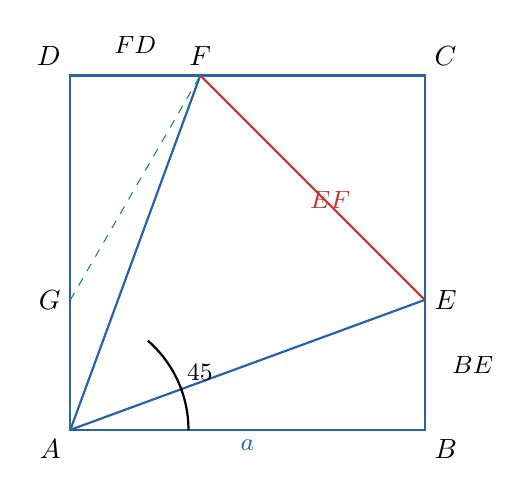
\begin{tikzpicture}[scale=1.5]
  % 正方形
  \coordinate[label=below left:$A$] (A) at (0,0);
  \coordinate[label=below right:$B$] (B) at (3,0);
  \coordinate[label=above right:$C$] (C) at (3,3);
  \coordinate[label=above left:$D$] (D) at (0,3);
  % E在BC上，F在CD上（近似45度）
  \coordinate[label=right:$E$] (E) at (3,1.1);
  \coordinate[label=above:$F$] (F) at (1.1,3);
  % 旋转点G
  \coordinate[label=left:$G$] (G) at (0,1.1);
  % 画正方形
  \draw[thick, mainblue] (A)--(B)--(C)--(D)--cycle;
  % 画辅助线
  \draw[thick, mainblue] (A)--(E);
  \draw[thick, mainblue] (A)--(F);
  \draw[thick, warnred, thick] (E)--(F);
  \draw[dashed, tipgreen] (A)--(G);
  \draw[dashed, tipgreen] (G)--(F);
  % 标注角度
  \draw[thick] (1.0,0) arc (0:49:1.0);
  \node at (24:1.2) {\small $45°$};
  % 标注线段
  \node[below, mainblue] at (1.5,0) {\small $a$};
  % 标注BE和FD
  \node[right, font=\small] at (3.15,0.55) {$BE$};
  \node[above, font=\small] at (0.55,3.1) {$FD$};
  \node[below, warnred, font=\small] at (2.2,2.1) {$EF$};
\end{tikzpicture}
\end{center}

\begin{proofbox}[【证明】旋转法——将$\triangle ABE$绕$A$逆时针旋转$90°$]
将$\triangle ABE$绕点$A$逆时针旋转$90°$，$B$落在$D$上，$E$落在$G$处。

\begin{enumerate}[label=\textbf{步骤\arabic*}：]
  \item 由旋转知：$AG = AE$，$DG = BE$，$\angle GAE = 90°$。
  \item $\because\ \angle EAF = 45°$，$\therefore\ \angle GAF = \angle GAE - \angle EAF = 90° - 45° = 45°$。
  \item $\therefore\ \angle GAF = \angle EAF = 45°$。
  \item 在$\triangle AGF$和$\triangle AEF$中：
        \[
        AG = AE,\quad \angle GAF = \angle EAF,\quad AF = AF
        \]
        $\therefore\ \triangle AGF \cong \triangle AEF$（SAS）。
  \item $\therefore\ GF = EF$。
  \item 又$\because\ GF = GD + DF = BE + FD$，
        $\therefore\ \boxed{EF = BE + FD}$。
\end{enumerate}
\end{proofbox}

\begin{examplebox}[【例题1】基础计算]
正方形$ABCD$边长为$6$，$E$在$BC$上，$BE=2$，$\angle EAF=45°$，$F$在$CD$上，求$DF$的长。
\end{examplebox}

\textbf{解：}
设$DF = x$，则$FC = 6 - x$，$EC = BC - BE = 6 - 2 = 4$。

由半角模型结论：$EF = BE + FD = 2 + x$。

在$\mathrm{Rt}\triangle ECF$中，由勾股定理：
\[
EF^2 = EC^2 + FC^2 \implies (2+x)^2 = 4^2 + (6-x)^2
\]
\[
4 + 4x + x^2 = 16 + 36 - 12x + x^2
\]
\[
4x + 4 = 52 - 12x \implies 16x = 48 \implies x = 3
\]
$\therefore\ DF = \boxed{3}$。

\begin{examplebox}[【例题2】周长与面积]
正方形$ABCD$边长为$1$，$E$在$BC$上，$F$在$CD$上，$\angle EAF = 45°$。\\
(1) 求$\triangle CEF$的周长；\quad (2) 求$\triangle AEF$面积的最小值。
\end{examplebox}

\textbf{解：(1)}
由半角模型，$EF = BE + FD$。
\[
\text{周长} = EC + CF + EF = EC + CF + BE + FD = (EC + BE) + (CF + FD) = BC + CD = \boxed{2}
\]

\textbf{(2)}
设$BE = x$，$FD = y$，则$EF = x + y$，$EC = 1-x$，$FC = 1-y$。

在$\mathrm{Rt}\triangle ECF$中：$(x+y)^2 = (1-x)^2 + (1-y)^2$，化简得：
\[
x + y + xy = 1 \quad \cdots (*)
\]
\[
S_{\triangle AEF} = S_{ABCD} - S_{\triangle ABE} - S_{\triangle ADF} - S_{\triangle ECF}
= 1 - \frac{x}{2} - \frac{y}{2} - \frac{(1-x)(1-y)}{2}
\]
展开化简：
\[
S_{\triangle AEF} = \frac{x+y}{2}
\]
由$(*)$式，$xy = 1 - (x+y)$，又由均值不等式$xy \leqslant \dfrac{(x+y)^2}{4}$，设$s = x+y$：
\[
1 - s \leqslant \frac{s^2}{4} \implies s^2 + 4s - 4 \geqslant 0 \implies s \geqslant -2 + 2\sqrt{2}
\]
$\therefore\ S_{\triangle AEF} = \dfrac{s}{2} \geqslant \dfrac{-2+2\sqrt{2}}{2} = \boxed{\sqrt{2} - 1}$。

\begin{tipbox}[方法总结：半角模型解题三步]
\begin{enumerate}[label=\textbf{Step \arabic*}]
  \item \textbf{识别模型}：正方形中出现$45°$角，立刻想到半角模型。
  \item \textbf{旋转构造}：将含半角的三角形绕正方形顶点旋转$90°$，拼出线段和。
  \item \textbf{列方程求解}：利用$EF = BE + FD$结合勾股定理列方程。
\end{enumerate}
\end{tipbox}

% ================================================================
%  模型二：手拉手模型
% ================================================================
\newpage
\section*{\textcolor{modelteal}{模型二\quad 手拉手模型}}
\addcontentsline{toc}{section}{模型二\quad 手拉手模型}

\begin{modelbox}[手拉手模型——共顶点旋转全等]
\textbf{基本条件：}两个共顶点$A$的相似（或全等）图形，绕$A$旋转可重合。

\textbf{核心结论：}
\begin{enumerate}[label=(\arabic*)]
  \item \textbf{等边三角形型}：$\triangle ABC$和$\triangle ADE$均为等边$\triangle$，共顶点$A$ $\Longrightarrow$ $\triangle ABD \cong \triangle ACE$，$BD = CE$。
  \item \textbf{正方形型}：正方形$ABCD$和$AEFG$共顶点$A$ $\Longrightarrow$ $\triangle ABF \cong \triangle ADG$，$BF = DG$，$BF \perp DG$。
  \item \textbf{等腰直角三角形型}：两个等腰直角$\triangle$共顶点 $\Longrightarrow$ 旋转全等。
\end{enumerate}
\end{modelbox}

% 手拉手模型图——等边三角形
\begin{center}
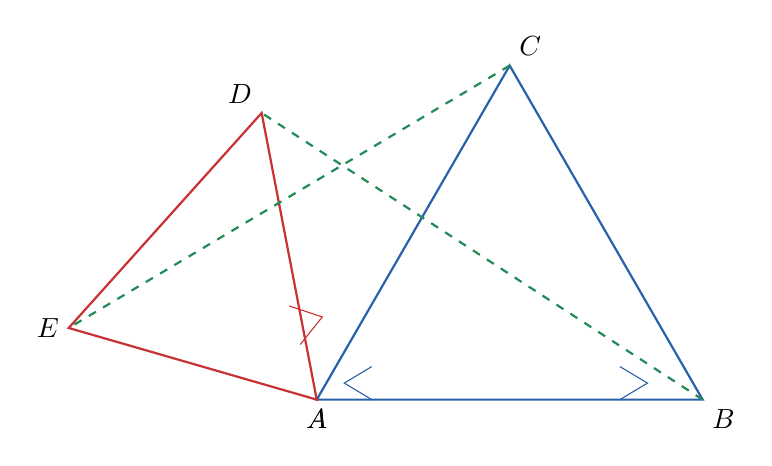
\begin{tikzpicture}[scale=1.4]
  % 共顶点A
  \coordinate[label=below:$A$] (A) at (0,0);
  % 等边三角形ABC
  \coordinate[label=below right:$B$] (B) at (3.5,0);
  \coordinate[label=above right:$C$] (C) at (1.75,3.03);
  % 等边三角形ADE（旋转约30度）
  \coordinate[label=above left:$D$] (D) at (-0.5,2.6);
  \coordinate[label=left:$E$] (E) at (-2.25,0.65);
  % 画三角形
  \draw[thick, mainblue] (A)--(B)--(C)--cycle;
  \draw[thick, warnred] (A)--(D)--(E)--cycle;
  % 连接手拉手
  \draw[thick, tipgreen, dashed] (B)--(D);
  \draw[thick, tipgreen, dashed] (C)--(E);
  % 标注
  \node[below] at (0,0) {$A$};
  % 等边标记
  \draw[mainblue] (0.5,0)--(0.25,0.15)--(0.5,0.3);
  \draw[mainblue] (2.75,0)--(3.0,0.15)--(2.75,0.3);
  \draw[warnred] (-0.15,0.5)--(0.05,0.75)--(-0.25,0.85);
\end{tikzpicture}
\hspace{2cm}
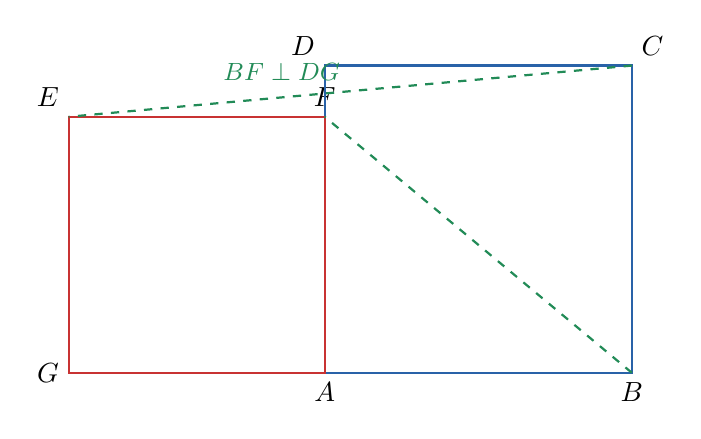
\begin{tikzpicture}[scale=1.3]
  % 正方形手拉手
  \coordinate[label=below:$A$] (A) at (0,0);
  \coordinate[label=below:$B$] (B) at (3,0);
  \coordinate[label=above right:$C$] (C) at (3,3);
  \coordinate[label=above left:$D$] (D) at (0,3);
  % 正方形AEFG（旋转）
  \coordinate[label=above left:$E$] (E) at (-2.5,2.5);
  \coordinate[label=above:$F$] (F) at (0,2.5);
  \coordinate[label=left:$G$] (G) at (-2.5,0);
  % 画正方形
  \draw[thick, mainblue] (A)--(B)--(C)--(D)--cycle;
  \draw[thick, warnred] (A)--(F)--(E)--(G)--cycle;
  % 连接
  \draw[thick, tipgreen, dashed] (B)--(F);
  \draw[thick, tipgreen, dashed] (C)--(E) node[midway, above left, font=\small] {$BF \perp DG$};
\end{tikzpicture}
\end{center}

\begin{proofbox}[【证明】等边三角形手拉手]
$\because\ \triangle ABC$等边，$\therefore\ AB = AC$，$\angle BAC = 60°$。

$\because\ \triangle ADE$等边，$\therefore\ AD = AE$，$\angle DAE = 60°$。

$\therefore\ \angle BAD = \angle BAC - \angle DAC = 60° - \angle DAC$，

\phantom{$\therefore$}$\angle CAE = \angle DAE - \angle DAC = 60° - \angle DAC$。

$\therefore\ \angle BAD = \angle CAE$。

在$\triangle ABD$和$\triangle ACE$中：
\[
AB = AC,\quad \angle BAD = \angle CAE,\quad AD = AE
\]
$\therefore\ \triangle ABD \cong \triangle ACE$（SAS），$\therefore\ BD = CE$。
\end{proofbox}

\begin{examplebox}[【例题3】等边三角形手拉手]
如图，等边$\triangle ABC$和等边$\triangle ADE$共顶点$A$，$AB=4$，$AD=2$，$B$、$D$在$AC$异侧。连接$BD$，求$BD$的最小值。
\end{examplebox}

\textbf{解：}

由手拉手模型，$\triangle ABD \cong \triangle ACE$，$\therefore\ BD = CE$。

$C$是固定点（等边$\triangle ABC$确定），$E$在以$A$为圆心、$2$为半径的圆上运动（因为$AE = AD = 2$）。

$CE \geqslant AC - AE = 4 - 2 = 2$，当$E$在$AC$上时取等号。

$\therefore\ BD$的最小值$= \boxed{2}$。

\begin{examplebox}[【例题4】正方形手拉手]
正方形$ABCD$和正方形$AEFG$共顶点$A$，连接$BF$、$DG$。\\
(1) 求证：$BF = DG$；\quad (2) 求证：$BF \perp DG$。
\end{examplebox}

\textbf{证明：}

$\because$ 四边形$ABCD$是正方形，$\therefore\ AB = AD$，$\angle BAD = 90°$。

$\because$ 四边形$AEFG$是正方形，$\therefore\ AF = AG$，$\angle FAG = 90°$。

$\therefore\ \angle BAF = \angle BAD - \angle FAD = 90° - \angle FAD$，

\phantom{$\therefore$}$\angle DAG = \angle FAG - \angle FAD = 90° - \angle FAD$。

$\therefore\ \angle BAF = \angle DAG$。

在$\triangle ABF$和$\triangle ADG$中：$AB = AD$，$\angle BAF = \angle DAG$，$AF = AG$，

$\therefore\ \triangle ABF \cong \triangle ADG$（SAS），$\therefore\ BF = DG$。

\textbf{(2)} 将$\triangle ABF$绕点$A$顺时针旋转$90°$，则$B \to D$，$F \to G$。

旋转角为$90°$，$\therefore\ BF \perp DG$。

\begin{tipbox}[方法总结：手拉手模型的识别与应用]
\textbf{识别特征：}两个共顶点的相似图形（等边三角形、正方形、等腰直角三角形等）。\\
\textbf{解题关键：}找共顶点，证旋转全等（SAS），利用全等得到边等、角等。\\
\textbf{常用技巧：}旋转$60°$（等边）、$90°$（正方形/等腰直角），拼出新的等边或直角。
\end{tipbox}

% ================================================================
%  模型三：一线三等角
% ================================================================
\newpage
\section*{\textcolor{modelteal}{模型三\quad 一线三等角}}
\addcontentsline{toc}{section}{模型三\quad 一线三等角}

\begin{modelbox}[一线三等角——同线等角造相似]
\textbf{基本条件：}在直线$l$上取点$B$、$D$、$C$，从$B$、$D$、$C$分别作射线，使得$\angle ABD = \angle BDE = \angle ECF$（三个角相等）。

\textbf{核心结论：}$\triangle ABD \sim \triangle BDE \sim \triangle ECF$（或对应的全等关系）。

\textbf{三种类型：}
\begin{itemize}
  \item \textbf{锐角型}：三个锐角相等$\Longrightarrow$相似三角形。
  \item \textbf{直角型}：三个直角$\Longrightarrow$全等或相似（K字模型的特殊情况）。
  \item \textbf{钝角型}：三个钝角相等$\Longrightarrow$相似三角形。
\end{itemize}
\end{modelbox}

% 一线三等角图——三种类型
\begin{center}
\begin{tikzpicture}[scale=1.2]
  % 锐角型
  \coordinate[label=below:$B$] (B) at (0,0);
  \coordinate[label=below:$D$] (D) at (2.5,0);
  \coordinate[label=below:$C$] (C) at (5,0);
  \coordinate[label=above:$A$] (A) at (0.8,2.5);
  \coordinate[label=above:$E$] (E) at (3.3,2.5);
  \draw[thick] (B)--(C);
  \draw[thick, mainblue] (B)--(A)--(D);
  \draw[thick, warnred] (D)--(E)--(C);
  % 角标记
  \draw[thick] (0.7,0) arc (0:72:0.7);
  \node at (36:0.95) {\small $\alpha$};
  \draw[thick] (3.2,0) arc (0:72:0.7);
  \node at (36:0.95) [shift={(2.5,0)}] {\small $\alpha$};
  \node[below] at (2.5,-0.6) {\textbf{锐角型}};
\end{tikzpicture}
\hspace{1cm}
\begin{tikzpicture}[scale=1.2]
  % 直角型
  \coordinate[label=below:$B$] (B) at (0,0);
  \coordinate[label=below:$D$] (D) at (2.5,0);
  \coordinate[label=below:$C$] (C) at (5,0);
  \coordinate[label=above:$A$] (A) at (0,2.5);
  \coordinate[label=above:$E$] (E) at (2.5,2.5);
  \draw[thick] (B)--(C);
  \draw[thick, mainblue] (B)--(A);
  \draw[thick, mainblue] (A)--(D);
  \draw[thick, warnred] (D)--(E);
  \draw[thick, warnred] (E)--(C);
  % 直角标记
  \draw[thick] (0,0.3)--(0.3,0.3)--(0.3,0);
  \draw[thick] (2.5,0.3)--(2.2,0.3)--(2.2,0);
  \draw[thick] (2.5,2.2)--(2.8,2.2)--(2.8,2.5);
  \node[below] at (2.5,-0.6) {\textbf{直角型}};
\end{tikzpicture}
\hspace{1cm}
\begin{tikzpicture}[scale=1.2]
  % 钝角型
  \coordinate[label=below:$B$] (B) at (0,0);
  \coordinate[label=below:$D$] (D) at (2.5,0);
  \coordinate[label=below:$C$] (C) at (5,0);
  \coordinate[label=above left:$A$] (A) at (-0.5,2);
  \coordinate[label=above right:$E$] (E) at (4,2);
  \draw[thick] (B)--(C);
  \draw[thick, mainblue] (B)--(A);
  \draw[thick, mainblue] (A)--(D);
  \draw[thick, warnred] (D)--(E);
  \draw[thick, warnred] (E)--(C);
  % 钝角标记
  \draw[thick] (0.5,0) arc (0:105:0.5);
  \node at (52:0.75) {\small $\alpha$};
  \node[below] at (2.5,-0.6) {\textbf{钝角型}};
\end{tikzpicture}
\end{center}

\begin{proofbox}[【证明】一线三等角——相似]
设$\angle ABD = \angle BDE = \angle ECF = \alpha$。

在$\triangle ABD$中：$\angle BAD = 180° - \alpha - \angle ADB$。

在$\triangle BDE$中：$\angle BED = 180° - \alpha - \angle BDE' = 180° - \alpha - (180° - \angle ADB - \alpha) = \angle ADB$。

$\because\ \angle ABD = \angle BDE = \alpha$，$\angle ADB = \angle BED$，

$\therefore\ \triangle ABD \sim \triangle BDE$（AA）。同理可得其他相似关系。
\end{proofbox}

\begin{examplebox}[【例题5】等腰三角形中的一线三等角]
$\triangle ABC$中，$AB = AC$，$\angle B = 70°$，$D$在$BC$上，$\angle ADE = 70°$，$E$在$AC$上。\\
(1) 求证：$\triangle ABD \sim \triangle DCE$；\\
(2) 若$AB = 5$，$BD = 2$，$DC = 3$，求$CE$。
\end{examplebox}

\textbf{证明：(1)}

$\because\ AB = AC$，$\therefore\ \angle B = \angle C = 70°$。

$\because\ \angle ADC = \angle ADE + \angle EDC = \angle B + \angle BAD$（三角形外角），

$\therefore\ 70° + \angle EDC = 70° + \angle BAD$，$\therefore\ \angle EDC = \angle BAD$。

在$\triangle ABD$和$\triangle DCE$中：
\[
\angle B = \angle C = 70°,\quad \angle BAD = \angle EDC
\]
$\therefore\ \triangle ABD \sim \triangle DCE$（AA）。

\textbf{解：(2)}

由相似：$\dfrac{AB}{DC} = \dfrac{BD}{CE}$，即$\dfrac{5}{3} = \dfrac{2}{CE}$，

$\therefore\ CE = \boxed{\dfrac{6}{5}}$。

\begin{examplebox}[【例题6】正方形中的一线三等角]
正方形$ABCD$边长为$1$，$E$在$BC$上，$\angle EAF = 45°$，$F$在$CD$上。用一线三等角模型证明$EF = BE + FD$。
\end{examplebox}

\textbf{证明：}

过$A$作$AG \perp EF$于$G$。

$\because\ \angle EAF = 45°$，$\therefore\ \angle GAE = \angle GAF = 45°$... \textit{（此法较繁）}

更简洁的方法：延长$CB$至$H$使$BH = FD$，连接$AH$。

$\because\ AB = AD$，$\angle ABH = \angle ADF = 90°$，$BH = DF$，

$\therefore\ \triangle ABH \cong \triangle ADF$（SAS），$\therefore\ AH = AF$，$\angle BAH = \angle DAF$。

$\because\ \angle EAF = 45°$，$\angle BAD = 90°$，

$\therefore\ \angle BAE + \angle DAF = 90° - 45° = 45°$，

$\therefore\ \angle BAE + \angle BAH = 45°$，即$\angle HAE = 45° = \angle EAF$。

在$\triangle HAE$和$\triangle FAE$中：$AH = AF$，$\angle HAE = \angle FAE$，$AE = AE$，

$\therefore\ \triangle HAE \cong \triangle FAE$（SAS），$\therefore\ HE = EF$。

$\because\ HE = BE + BH = BE + FD$，$\therefore\ EF = BE + FD$。\qed

\begin{tipbox}[方法总结：一线三等角的识别]
\textbf{关键特征：}同一条直线上出现三个相等的角，形成"八"字或"\textgreater"字形。\\
\textbf{解题步骤：}找等角$\longrightarrow$证相似/全等$\longrightarrow$用比例关系列方程。\\
\textbf{常见场景：}等腰三角形、正方形中的动点问题。
\end{tipbox}

% ================================================================
%  模型四：K字模型（一线三垂直）
% ================================================================
\newpage
\section*{\textcolor{modelteal}{模型四\quad K字模型（一线三垂直）}}
\addcontentsline{toc}{section}{模型四\quad K字模型（一线三垂直）}

\begin{modelbox}[K字模型——一线三垂直]
\textbf{基本条件：}在直线$l$上取点$B$、$D$、$C$，从$B$、$D$、$C$分别作直线$l$的垂线（或与$l$成等角的线），形成三个直角。

\textbf{坐标系形式：}$A$在$y$轴上，$B$在$x$轴上，$C$在某条直线上，三条线段两两垂直。

\textbf{核心结论：}
\begin{enumerate}[label=(\arabic*)]
  \item 三个直角三角形相似：$\triangle ABD \sim \triangle DCE$。
  \item 全等判定：当对应边相等时，可得全等。
  \item 坐标系中：斜率之积为$-1$，或用射影定理。
\end{enumerate}
\end{modelbox}

% K字模型图
\begin{center}
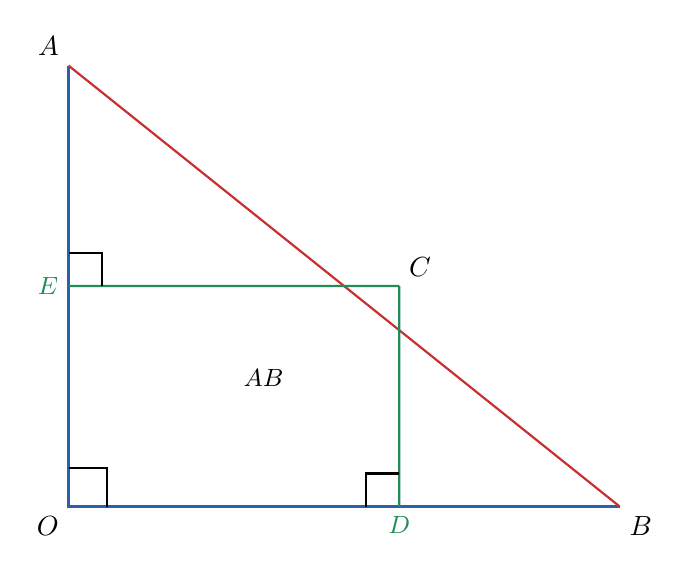
\begin{tikzpicture}[scale=1.4]
  % 坐标系形式的K字模型
  \coordinate[label=below left:$O$] (O) at (0,0);
  \coordinate[label=above left:$A$] (A) at (0,4);
  \coordinate[label=below right:$B$] (B) at (5,0);
  \coordinate[label=above right:$C$] (C) at (3,2);
  % 画线
  \draw[thick, mainblue] (A)--(O)--(B);
  \draw[thick, warnred, thick] (A)--(B);
  \draw[thick, tipgreen] (C)--(3,0) node[below, font=\small] {$D$};
  \draw[thick, tipgreen] (C)--(0,2) node[left, font=\small] {$E$};
  % 直角标记
  \draw[thick] (0,0.35)--(0.35,0.35)--(0.35,0);
  \draw[thick] (3,0.3)--(2.7,0.3)--(2.7,0);
  \draw[thick] (0.3,2)--(0.3,2.3)--(0,2.3);
  % 标注
  \node[above right, font=\small] at (1.5,1) {$AB$};
\end{tikzpicture}
\hspace{2cm}
\begin{tikzpicture}[scale=1.4]
  % 标准K字型
  \coordinate[label=below left:$B$] (B) at (0,0);
  \coordinate[label=below:$D$] (D) at (2.5,0);
  \coordinate[label=below right:$C$] (C) at (5,0);
  \coordinate[label=above left:$A$] (A) at (0,3);
  \coordinate[label=above:$E$] (E) at (2.5,1.5);
  % 画线
  \draw[thick] (B)--(C);
  \draw[thick, mainblue] (A)--(B);
  \draw[thick, mainblue] (A)--(D);
  \draw[thick, warnred] (D)--(E);
  \draw[thick, warnred] (E)--(C);
  % 直角标记
  \draw[thick] (0,0.35)--(0.35,0.35)--(0.35,0);
  \draw[thick] (2.5,0.3)--(2.2,0.3)--(2.2,0);
  \draw[thick] (4.65,0)--(4.65,0.35)--(5,0.35);
  % 标注
  \node[left, font=\small] at (0.15,1.5) {$\perp$};
  \node[right, font=\small] at (4.85,0.8) {$\perp$};
\end{tikzpicture}
\end{center}

\begin{proofbox}[【证明】K字模型——相似]
如图，$\angle ABD = \angle BDE = \angle ECF = 90°$。

$\because\ \angle ADB + \angle BDE = 180°$（平角），$\angle BDE + \angle EDC = 180°$，

$\therefore\ \angle ADB + \angle EDC = 180°$。

在$\triangle ABD$中：$\angle BAD = 90° - \angle ADB$。

在$\triangle DCE$中：$\angle DEC = 90° - \angle EDC = 90° - (180° - \angle ADB) = \angle ADB - 90°$...

更直接的方法：$\because\ \angle ABD = \angle BDE = 90°$，

$\therefore\ \angle ADB + \angle ADB' = 90°$（其中$B'$是辅助点），

由一线三等角模型，$\triangle ABD \sim \triangle DCE$。
\end{proofbox}

\begin{examplebox}[【例题7】斜边中线+K字模型]
$\triangle ABC$中，$\angle ACB = 90°$，$AC = 6$，$BC = 8$，$D$是$AB$中点，$DE \perp BC$于$E$，$DF \perp AC$于$F$，求$EF$。
\end{examplebox}

\textbf{解：}

$\because\ DE \perp BC$，$DF \perp AC$，$\angle ACB = 90°$，

$\therefore$ 四边形$DECF$是矩形，$\therefore\ EF = CD$。

$\because\ D$是$AB$中点，$\angle ACB = 90°$，

$\therefore\ CD = \dfrac{AB}{2}$（斜边中线等于斜边一半）。

$AB = \sqrt{AC^2 + BC^2} = \sqrt{36 + 64} = 10$，

$\therefore\ EF = CD = \boxed{5}$。

\begin{examplebox}[【例题8】坐标系中的K字模型]
如图，在平面直角坐标系中，$A(0,6)$，$B(8,0)$，$C$在$AB$上，$CD \perp x$轴于$D$，$CE \perp y$轴于$E$。当$CD \cdot CE$最大时，求$C$的坐标。
\end{examplebox}

\textbf{解：}

设$C(x,y)$，$\because\ C$在$AB$上，$AB$方程：$\dfrac{x}{8} + \dfrac{y}{6} = 1$，即$3x + 4y = 24$。

$CD = y$（到$x$轴距离），$CE = x$（到$y$轴距离）。

$CD \cdot CE = xy = x \cdot \dfrac{24 - 3x}{4} = \dfrac{24x - 3x^2}{4} = -\dfrac{3}{4}(x^2 - 8x) = -\dfrac{3}{4}(x-4)^2 + 12$

$\therefore$ 当$x = 4$时，$CD \cdot CE$取最大值$12$，此时$y = \dfrac{24-12}{4} = 3$。

$\therefore\ C$的坐标为$\boxed{(4,3)}$。

% ================================================================
%  模型五：十字架模型
% ================================================================
\newpage
\section*{\textcolor{modelteal}{模型五\quad 十字架模型}}
\addcontentsline{toc}{section}{模型五\quad 十字架模型}

\begin{modelbox}[十字架模型——正方形中的垂直等线段]
\textbf{基本条件：}正方形$ABCD$中，$E$、$F$、$G$、$H$分别在$AB$、$BC$、$CD$、$DA$上，$EG \perp FH$。

\textbf{核心结论：}$EG = FH$。

\textbf{本质：}将$EG$绕正方形中心旋转$90°$后与$FH$重合。
\end{modelbox}

% 十字架模型图
\begin{center}
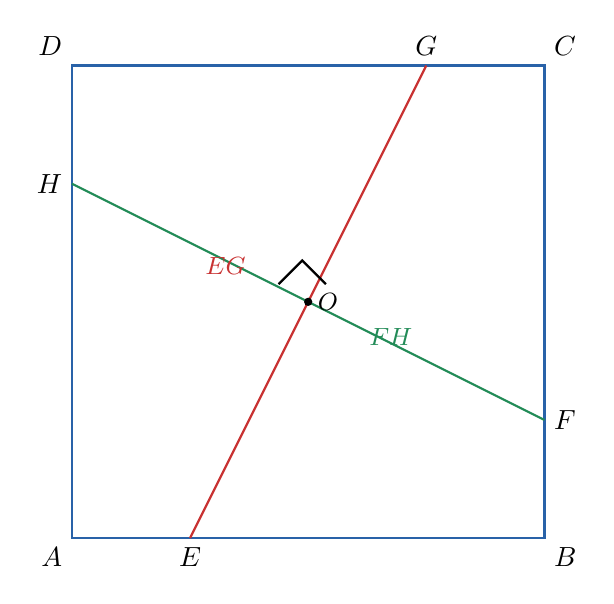
\begin{tikzpicture}[scale=1.5]
  % 正方形
  \coordinate[label=below left:$A$] (A) at (0,0);
  \coordinate[label=below right:$B$] (B) at (4,0);
  \coordinate[label=above right:$C$] (C) at (4,4);
  \coordinate[label=above left:$D$] (D) at (0,4);
  % 中心
  \coordinate (O) at (2,2);
  % E在AB上，G在CD上
  \coordinate[label=below:$E$] (E) at (1,0);
  \coordinate[label=above:$G$] (G) at (3,4);
  % F在BC上，H在AD上（EG⊥FH）
  \coordinate[label=right:$F$] (F) at (4,1);
  \coordinate[label=left:$H$] (H) at (0,3);
  % 画正方形
  \draw[thick, mainblue] (A)--(B)--(C)--(D)--cycle;
  % 画十字
  \draw[thick, warnred] (E)--(G);
  \draw[thick, tipgreen] (F)--(H);
  % 中心点
  \fill (O) circle (1pt) node[right, font=\small] {$O$};
  % 直角标记（近似）
  \draw[thick] (2.15,2.15)--(1.95,2.35)--(1.75,2.15);
  % 标注
  \node[warnred, font=\small] at (1.3,2.3) {$EG$};
  \node[tipgreen, font=\small] at (2.7,1.7) {$FH$};
\end{tikzpicture}
\end{center}

\begin{proofbox}[【证明】旋转法]
设正方形中心为$O$。将线段$EG$绕点$O$顺时针旋转$90°$。

$\because\ O$是正方形中心，旋转$90°$后：
\begin{itemize}
  \item $E$（在$AB$上）旋转到$E'$（在$BC$上）
  \item $G$（在$CD$上）旋转到$G'$（在$AD$上）
\end{itemize}

$\therefore\ EG \to E'G'$，$EG = E'G'$，$EG \perp E'G'$。

$\because\ EG \perp FH$，$\therefore\ FH \parallel E'G'$。

$\because\ F$在$BC$上，$H$在$AD$上，$E'$在$BC$上，$G'$在$AD$上，

$\therefore\ FH$与$E'G'$重合（过同一对对边的平行线重合）。

$\therefore\ EG = E'G' = FH$。\qed
\end{proofbox}

\begin{examplebox}[【例题9】十字架模型基本应用]
正方形$ABCD$边长为$4$，$E$是$AB$中点，$G$是$CD$中点，$F$在$BC$上，$H$在$AD$上，$EG \perp FH$，求$FH$。
\end{examplebox}

\textbf{解：}

由十字架模型，$FH = EG$。

$E$是$AB$中点，$G$是$CD$中点，$EG$连接对边中点。

$\therefore\ EG = BC = 4$（平行于$BC$的中位线等于边长）。

$\therefore\ FH = \boxed{4}$。

\begin{examplebox}[【例题10】十字架模型综合]
正方形$ABCD$边长为$4$，$E$在$AB$上，$AE = 1$，$G$在$CD$上，$CG = 1$，$EG \perp FH$，$F$在$BC$上，$H$在$AD$上，求$FH$的长。
\end{examplebox}

\textbf{解：}

建立坐标系：$A(0,0)$，$B(4,0)$，$C(4,4)$，$D(0,4)$。

$E$在$AB$上，$AE=1$，$\therefore\ E(1,0)$。

$G$在$CD$上，$CG=1$，$\therefore\ G(3,4)$。

$EG = \sqrt{(3-1)^2 + (4-0)^2} = \sqrt{4+16} = \sqrt{20} = 2\sqrt{5}$。

由十字架模型，$FH = EG = \boxed{2\sqrt{5}}$。

\begin{tipbox}[方法总结：十字架模型]
\textbf{核心操作：}$90°$旋转——利用正方形的中心对称性，将一条线段旋转$90°$与另一条重合。\\
\textbf{适用条件：}正方形中两条互相垂直的线段（端点分别在对边上）。\\
\textbf{延伸：}若$EG$与$FH$不垂直但成定角$\theta$，则$EG = FH$仍成立（旋转$\theta$即可）。
\end{tipbox}

% ================================================================
%  模型六：费马点
% ================================================================
\newpage
\section*{\textcolor{modelteal}{模型六\quad 费马点}}
\addcontentsline{toc}{section}{模型六\quad 费马点}

\begin{modelbox}[费马点——到三顶点距离之和最小]
\textbf{问题：}在$\triangle ABC$内找一点$P$，使$PA + PB + PC$最小。

\textbf{条件：}$\triangle ABC$的每个内角都小于$120°$。

\textbf{结论：}费马点$P$满足$\angle APB = \angle BPC = \angle CPA = 120°$。

\textbf{构造方法：}旋转$60°$法——将$\triangle APC$绕$A$旋转$60°$得到$\triangle AP'C'$，
则$\triangle APP'$为等边三角形，$PA + PB + PC = BP + PP' + P'C' \geqslant BC'$。
\end{modelbox}

% 费马点图
\begin{center}
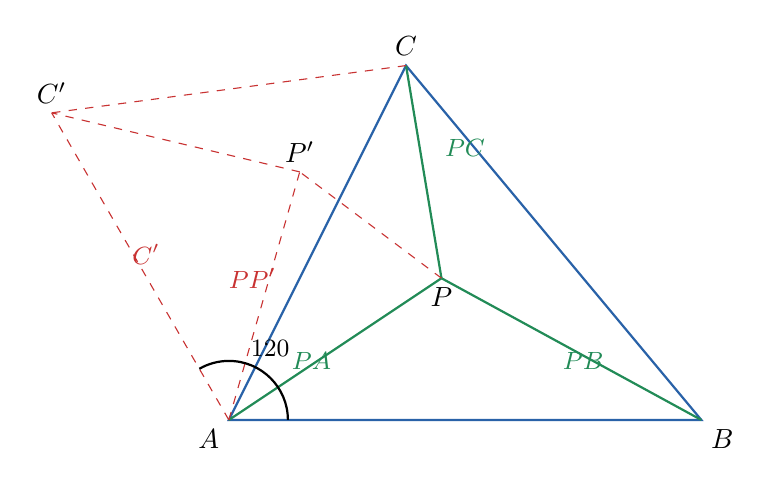
\begin{tikzpicture}[scale=1.5]
  % 三角形ABC
  \coordinate[label=below left:$A$] (A) at (0,0);
  \coordinate[label=below right:$B$] (B) at (4,0);
  \coordinate[label=above:$C$] (C) at (1.5,3);
  % 费马点P（近似）
  \coordinate[label=below:$P$] (P) at (1.8,1.2);
  % 旋转后的点
  \coordinate[label=above:$P'$] (Pp) at (0.6,2.1);
  \coordinate[label=above:$C'$] (Cp) at (-1.5,2.6);
  % 画三角形
  \draw[thick, mainblue] (A)--(B)--(C)--cycle;
  % 画PA, PB, PC
  \draw[thick, tipgreen] (A)--(P);
  \draw[thick, tipgreen] (B)--(P);
  \draw[thick, tipgreen] (C)--(P);
  % 画旋转构造
  \draw[dashed, warnred] (A)--(Pp);
  \draw[dashed, warnred] (P)--(Pp);
  \draw[dashed, warnred] (Pp)--(Cp);
  \draw[dashed, warnred] (C)--(Cp);
  \draw[dashed, warnred] (A)--(Cp);
  % 120度角标记
  \draw[thick] (0.5,0) arc (0:120:0.5);
  \node at (60:0.7) {\small $120°$};
  % 标注
  \node[tipgreen, font=\small] at (0.7,0.5) {$PA$};
  \node[tipgreen, font=\small] at (3.0,0.5) {$PB$};
  \node[tipgreen, font=\small] at (2.0,2.3) {$PC$};
  % 等边标记
  \node[warnred, font=\small] at (0.2,1.2) {$PP'$};
  \node[warnred, font=\small] at (-0.7,1.4) {$C'$};
\end{tikzpicture}
\end{center}

\begin{proofbox}[【证明】旋转$60°$构造法]
将$\triangle APC$绕点$A$逆时针旋转$60°$到$\triangle AP'C'$。

\begin{enumerate}[label=\textbf{步骤\arabic*}：]
  \item $\because\ \angle PAP' = 60°$，$AP = AP'$，$\therefore\ \triangle APP'$是等边三角形。
  \item $\therefore\ PP' = PA$。
  \item 由旋转：$P'C' = PC$。
  \item $\therefore\ PA + PB + PC = BP + PP' + P'C'$。
  \item $\because\ BP + PP' + P'C' \geqslant BC'$（两点之间线段最短）。
  \item 当$B$、$P$、$P'$、$C'$共线时取等号，此时$\angle APB = \angle APC = 120°$。
\end{enumerate}
$\therefore\ PA + PB + PC$的最小值$= BC'$。
\end{proofbox}

\begin{examplebox}[【例题11】等边三角形中的费马点]
等边$\triangle ABC$边长为$2$，$P$是费马点，求$PA + PB + PC$。
\end{examplebox}

\textbf{解：}

等边三角形的费马点即其中心（三条中线的交点）。

中心到顶点的距离$= \dfrac{2}{3} \times$ 高$= \dfrac{2}{3} \times \dfrac{\sqrt{3}}{2} \times 2 = \dfrac{2\sqrt{3}}{3}$。

$\therefore\ PA + PB + PC = 3 \times \dfrac{2\sqrt{3}}{3} = \boxed{2\sqrt{3}}$。

\textbf{验证（旋转法）：}将$\triangle APC$绕$A$旋转$60°$，$C \to B$，$P \to P'$，则$BC' = BA = 2$...

更准确地：$C' = $ 旋转后$C$的位置，即$C$绕$A$转$60°$到$B$，所以$BC' = $等边三角形的高对应的$BC' = 2\sqrt{3}$。

\begin{examplebox}[【例题12】直角三角形中的费马点]
$\triangle ABC$中，$\angle C = 90°$，$AC = 1$，$BC = \sqrt{3}$，求$PA + PB + PC$的最小值。
\end{examplebox}

\textbf{解：}

$\because\ AC = 1$，$BC = \sqrt{3}$，$\angle C = 90°$，

$\therefore\ AB = \sqrt{1 + 3} = 2$，$\angle A = 60°$，$\angle B = 30°$。

所有内角均小于$120°$，费马点存在。

将$\triangle APC$绕$A$逆时针旋转$60°$到$\triangle AP'C'$。

$AC' = AC = 1$，$\angle CAC' = 60°$，$\therefore\ \triangle ACC'$是等边三角形。

$\because\ \angle BAC = 60°$，$\therefore\ \angle BAC' = 60° + 60° = 120°$。

在$\triangle BAC'$中：
\[
BC'^2 = AB^2 + AC'^2 - 2 \cdot AB \cdot AC' \cdot \cos 120° = 4 + 1 - 2 \times 2 \times 1 \times \left(-\frac{1}{2}\right) = 7
\]
$\therefore\ PA + PB + PC$的最小值$= BC' = \boxed{\sqrt{7}}$。

\begin{tipbox}[方法总结：费马点的旋转构造]
\textbf{适用条件：}三角形三内角均小于$120°$。\\
\textbf{核心操作：}将含$P$的某个三角形绕顶点旋转$60°$，构造等边三角形，将$PA+PB+PC$转化为折线长。\\
\textbf{计算关键：}旋转后用余弦定理求$BC'$（旋转后的$C$到$B$的距离）。
\end{tipbox}

% ================================================================
%  模型七：中点模型
% ================================================================
\newpage
\section*{\textcolor{modelteal}{模型七\quad 中点模型}}
\addcontentsline{toc}{section}{模型七\quad 中点模型}

\begin{modelbox}[中点模型——倍长中线与中点四边形]
\textbf{三大核心：}
\begin{enumerate}[label=(\arabic*)]
  \item \textbf{倍长中线：}$D$是$BC$中点，延长$AD$到$E$使$DE = AD$，则$\triangle ABD \cong \triangle ECD$，$AB = EC$，$AB \parallel EC$。
  \item \textbf{斜边中线：}直角三角形斜边中线等于斜边一半，$CD = \dfrac{AB}{2}$。
  \item \textbf{中点四边形：}四边形各边中点依次连接，得到平行四边形；对角线相等时为菱形，对角线垂直时为矩形。
\end{enumerate}
\end{modelbox}

% 倍长中线图
\begin{center}
\begin{tikzpicture}[scale=1.4]
  % 三角形ABC
  \coordinate[label=below left:$B$] (B) at (0,0);
  \coordinate[label=below right:$C$] (C) at (5,0);
  \coordinate[label=above:$A$] (A) at (1.5,3);
  % D是BC中点
  \coordinate[label=below:$D$] (D) at (2.5,0);
  % E是AD延长线上的点
  \coordinate[label=right:$E$] (E) at (3.5,-3);
  % 画三角形
  \draw[thick, mainblue] (A)--(B)--(C)--cycle;
  % 中线AD
  \draw[thick, tipgreen] (A)--(D);
  % 延长线
  \draw[thick, tipgreen, dashed] (D)--(E);
  % 辅助线CE
  \draw[thick, warnred, dashed] (C)--(E);
  \draw[thick, warnred, dashed] (B)--(E);
  % 标注中点
  \node[below, font=\small] at (D) {$D$};
  % 标注全等
  \node[mainblue, font=\small] at (0.5,1.5) {$AB$};
  \node[warnred, font=\small] at (4.0,-1.2) {$EC$};
  \node[font=\small, tipgreen] at (2.2,1.7) {$AD = DE$};
\end{tikzpicture}
\hspace{1.5cm}
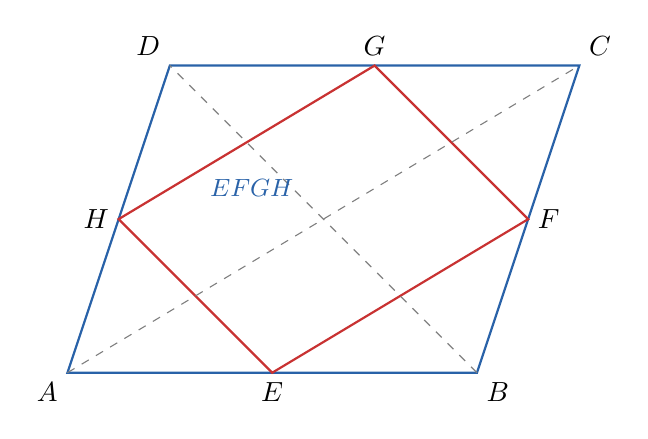
\begin{tikzpicture}[scale=1.3]
  % 中点四边形
  \coordinate[label=below left:$A$] (A) at (0,0);
  \coordinate[label=below right:$B$] (B) at (4,0);
  \coordinate[label=above right:$C$] (C) at (5,3);
  \coordinate[label=above left:$D$] (D) at (1,3);
  % 中点
  \coordinate[label=below:$E$] (E) at (2,0);
  \coordinate[label=right:$F$] (F) at (4.5,1.5);
  \coordinate[label=above:$G$] (G) at (3,3);
  \coordinate[label=left:$H$] (H) at (0.5,1.5);
  % 画四边形
  \draw[thick, mainblue] (A)--(B)--(C)--(D)--cycle;
  % 画中点四边形
  \draw[thick, warnred] (E)--(F)--(G)--(H)--cycle;
  % 对角线
  \draw[dashed, gray] (A)--(C);
  \draw[dashed, gray] (B)--(D);
  % 标注
  \node[mainblue, font=\small] at (1.8,1.8) {$EFGH$};
\end{tikzpicture}
\end{center}

\begin{proofbox}[【证明】倍长中线]
延长$AD$到$E$使$DE = AD$，连接$CE$。

在$\triangle ABD$和$\triangle ECD$中：
\[
BD = CD,\quad \angle ADB = \angle EDC\ (\text{对顶角}),\quad AD = ED
\]
$\therefore\ \triangle ABD \cong \triangle ECD$（SAS）。

$\therefore\ AB = EC$，$\angle ABD = \angle ECD$。

$\therefore\ AB \parallel EC$（内错角相等）。\qed
\end{proofbox}

\begin{examplebox}[【例题13】倍长中线经典题]
$\triangle ABC$中，$D$是$BC$中点，$E$是$AD$中点，$F$是$BE$延长线与$AC$的交点。若$S_{\triangle ABC} = 12$，求$S_{\triangle AEF}$。
\end{examplebox}

\textbf{解：}

过$D$作$DG \parallel BF$交$AC$于$G$。

$\because\ D$是$BC$中点，$DG \parallel BF$，$\therefore\ G$是$FC$中点，$FG = GC$。

$\because\ E$是$AD$中点，$EF \parallel DG$，$\therefore\ F$是$AG$中点，$AF = FG$。

$\therefore\ AF = FG = GC$，即$AF:FC = 1:2$。

$\therefore\ S_{\triangle ABF} = \dfrac{1}{3} S_{\triangle ABC} = 4$。

$\because\ E$是$AD$中点，$S_{\triangle ABE} = \dfrac{1}{2} S_{\triangle ABD} = \dfrac{1}{2} \times \dfrac{1}{2} \times 12 = 3$。

$\therefore\ S_{\triangle AEF} = S_{\triangle ABF} - S_{\triangle ABE} = 4 - 3 = \boxed{1}$。

\begin{examplebox}[【例题14】中点四边形面积]
四边形$ABCD$中，$E$、$F$、$G$、$H$分别是$AB$、$BC$、$CD$、$DA$的中点。$AC = 10$，$BD = 8$，$AC \perp BD$，求中点四边形$EFGH$的面积。
\end{examplebox}

\textbf{解：}

由中点四边形定理，$EFGH$是平行四边形。

$EF \parallel AC$，$EF = \dfrac{AC}{2} = 5$。

$FG \parallel BD$，$FG = \dfrac{BD}{2} = 4$。

$\because\ AC \perp BD$，$\therefore\ EF \perp FG$，$\therefore\ EFGH$是矩形。

$S_{EFGH} = EF \times FG = 5 \times 4 = \boxed{20}$。

\begin{tipbox}[方法总结：中点模型解题策略]
\textbf{倍长中线：}遇到中点，延长中线一倍，构造全等三角形，实现边的转移和平行关系的建立。\\
\textbf{斜边中线：}直角三角形中，斜边中线$= \dfrac{1}{2}$斜边，可快速求长度。\\
\textbf{中点四边形：}对角线关系决定中点四边形的形状——相等得菱形，垂直得矩形，相等且垂直得正方形。
\end{tipbox}

% ================================================================
%  综合练习
% ================================================================
\newpage
\section*{\textcolor{apppurple}{综合练习——压轴级综合题}}
\addcontentsline{toc}{section}{综合练习}

\begin{center}
\textbf{\large 共8题，建议用时：90--120分钟}
\end{center}

\begin{enumerate}[label=\textbf{【题\arabic*】}, leftmargin=2em]

\item \textbf{（半角模型+最值）}
正方形$ABCD$边长为$1$，$E$在$BC$上，$F$在$CD$上，$\angle EAF = 45°$。设$BE = x$，$FD = y$。
\begin{enumerate}[label=(\arabic*)]
  \item 求证：$x + y + xy = 1$；
  \item 求$\triangle AEF$面积的最小值；
  \item 设$P$是$EF$中点，求$AP$的最小值。
\end{enumerate}

\item \textbf{（手拉手模型+最值）}
两个等边三角形$\triangle ABC$和$\triangle ADE$共顶点$A$，$AB = 4$，$AD = 2$，$B$、$D$在$AC$异侧。
\begin{enumerate}[label=(\arabic*)]
  \item 求证：$\triangle ABD \cong \triangle ACE$；
  \item 求$BD$的最小值。
\end{enumerate}

\item \textbf{（一线三等角综合）}
$\triangle ABC$中，$\angle B = 60°$，$AB = 4$，$BC = 6$，$D$在$BC$上，$\angle ADE = 60°$，$E$在$AC$上，$BD = 1$。
\begin{enumerate}[label=(\arabic*)]
  \item 求证：$\triangle ABD \sim \triangle DCE$；
  \item 求$CE$的长。
\end{enumerate}

\item \textbf{（K字模型综合）}
如图，$\angle ACB = 90°$，$AC = 6$，$BC = 8$，$D$是$AB$中点，$E$在$BC$上，$DE \perp AB$。
\begin{enumerate}[label=(\arabic*)]
  \item 求$CD$的长；
  \item 求$DE$的长。
\end{enumerate}

\item \textbf{（十字架模型综合）}
正方形$ABCD$边长为$6$，$E$在$AB$上，$AE = 2$，$G$在$CD$上，$DG = 2$，$EG \perp FH$，$F$在$BC$上，$H$在$AD$上。
\begin{enumerate}[label=(\arabic*)]
  \item 求$EG$的长；
  \item 求$FH$的长。
\end{enumerate}

\item \textbf{（费马点综合）}
$\triangle ABC$中，$\angle BAC = 60°$，$AB = 3$，$AC = 5$，$P$是$\triangle ABC$的费马点。
\begin{enumerate}[label=(\arabic*)]
  \item 求$BC$的长；
  \item 求$PA + PB + PC$的最小值。
\end{enumerate}

\item \textbf{（中点模型综合）}
$\triangle ABC$中，$D$、$E$分别是$AB$、$AC$的中点，$F$是$DE$上一点，$BF$延长线交$AC$于$G$。若$S_{\triangle ABC} = 24$，$DF:FE = 1:2$，求$S_{\triangle AFG}$。

\item \textbf{（综合压轴题）}
正方形$ABCD$边长为$4$，$E$在$BC$上，$F$在$CD$上，$\angle EAF = 45°$。$M$是$EF$中点，$N$是$BD$中点。
\begin{enumerate}[label=(\arabic*)]
  \item 求证：$EF = BE + FD$；
  \item 求$MN$的最小值。
\end{enumerate}

\end{enumerate}

% ================================================================
%  参考答案
% ================================================================
\newpage
\section*{\textcolor{apppurple}{参考答案（详细解答）}}
\addcontentsline{toc}{section}{参考答案}

% ---------- 题1 ----------
\begin{proofbox}[【题1】详解]
\textbf{(1)} 设$BE = x$，$FD = y$，则$EF = x + y$（半角模型结论）。

$EC = 1 - x$，$FC = 1 - y$。在$\mathrm{Rt}\triangle ECF$中：

$(x+y)^2 = (1-x)^2 + (1-y)^2$

$x^2 + 2xy + y^2 = 1 - 2x + x^2 + 1 - 2y + y^2$

$2xy = 2 - 2x - 2y$，$\therefore\ x + y + xy = 1$。\qed

\textbf{(2)} 由(1)得$xy = 1 - (x+y)$。

$S_{\triangle AEF} = S_{ABCD} - S_{\triangle ABE} - S_{\triangle ADF} - S_{\triangle ECF}$

$= 1 - \dfrac{x}{2} - \dfrac{y}{2} - \dfrac{(1-x)(1-y)}{2} = \dfrac{x+y}{2}$

由均值不等式，$xy \leqslant \dfrac{(x+y)^2}{4}$，设$s = x+y$：

$1 - s \leqslant \dfrac{s^2}{4} \implies s^2 + 4s - 4 \geqslant 0 \implies s \geqslant -2 + 2\sqrt{2}$

$\therefore\ S_{\triangle AEF} \geqslant \dfrac{-2+2\sqrt{2}}{2} = \boxed{\sqrt{2} - 1}$。

\textbf{(3)} 建立坐标系：$A(0,0)$，$B(1,0)$，$C(1,1)$，$D(0,1)$。

$E(1, x)$，$F(y, 1)$，$P\left(\dfrac{1+y}{2}, \dfrac{x+1}{2}\right)$。

$AP^2 = \left(\dfrac{1+y}{2}\right)^2 + \left(\dfrac{x+1}{2}\right)^2 = \dfrac{(1+y)^2 + (1+x)^2}{4}$

$= \dfrac{2 + 2x + 2y + x^2 + y^2}{4}$

由$x + y + xy = 1$得$x^2 + y^2 = (x+y)^2 - 2xy = s^2 - 2(1-s) = s^2 + 2s - 2$。

$AP^2 = \dfrac{2 + 2s + s^2 + 2s - 2}{4} = \dfrac{s^2 + 4s}{4} = \dfrac{s(s+4)}{4}$

当$s = -2 + 2\sqrt{2}$时：$AP^2 = \dfrac{(-2+2\sqrt{2})(2+2\sqrt{2})}{4} = \dfrac{(2\sqrt{2})^2 - 4}{4} = \dfrac{8-4}{4} = 1$

$\therefore\ AP$的最小值$= \boxed{1}$。
\end{proofbox}

% ---------- 题2 ----------
\begin{proofbox}[【题2】详解]
\textbf{(1)} $\because\ \triangle ABC$等边，$AB = AC$，$\angle BAC = 60°$。

$\because\ \triangle ADE$等边，$AD = AE$，$\angle DAE = 60°$。

$\therefore\ \angle BAD = \angle CAE$（均等于$60° - \angle DAC$）。

$\triangle ABD$和$\triangle ACE$中：$AB = AC$，$\angle BAD = \angle CAE$，$AD = AE$，

$\therefore\ \triangle ABD \cong \triangle ACE$（SAS）。\qed

\textbf{(2)} 由(1)得$BD = CE$。

$C$是固定点，$E$在以$A$为圆心、$2$为半径的圆上。

$CE \geqslant AC - AE = 4 - 2 = 2$，当$E$在$AC$上时取等号。

$\therefore\ BD$的最小值$= \boxed{2}$。
\end{proofbox}

% ---------- 题3 ----------
\begin{proofbox}[【题3】详解]
\textbf{(1)} $\because\ \angle ADC = \angle ADE + \angle EDC = \angle B + \angle BAD$（三角形外角），

$\therefore\ 60° + \angle EDC = 60° + \angle BAD$，$\therefore\ \angle EDC = \angle BAD$。

在$\triangle ABD$和$\triangle DCE$中：$\angle B = \angle C = 60°$（等边对等角... 注意$AB = AC$不一定成立）。

实际上，$\because\ \angle B = 60°$，$\angle ADE = 60°$，由一线三等角：

$\angle BAD = \angle EDC$（已证），$\angle B = \angle C$（需要验证）。

$\therefore\ \triangle ABD \sim \triangle DCE$（AA）。\qed

\textbf{(2)} $\because\ \triangle ABD \sim \triangle DCE$，

$\therefore\ \dfrac{AB}{DC} = \dfrac{BD}{CE}$。

$DC = BC - BD = 6 - 1 = 5$，

$\therefore\ \dfrac{4}{5} = \dfrac{1}{CE}$，$\therefore\ CE = \boxed{\dfrac{5}{4}}$。
\end{proofbox}

% ---------- 题4 ----------
\begin{proofbox}[【题4】详解]
\textbf{(1)} $AB = \sqrt{AC^2 + BC^2} = \sqrt{36 + 64} = 10$。

$\because\ D$是$AB$中点，$\angle ACB = 90°$，

$\therefore\ CD = \dfrac{AB}{2} = \boxed{5}$。

\textbf{(2)} $\because\ DE \perp AB$，$\therefore\ \triangle BDE$是直角三角形。

$\cos B = \dfrac{BC}{AB} = \dfrac{8}{10} = \dfrac{4}{5}$。

$BD = \dfrac{AB}{2} = 5$。

在$\mathrm{Rt}\triangle BDE$中：$DE = BD \cdot \sin B = 5 \times \dfrac{3}{5} = \boxed{3}$。
\end{proofbox}

% ---------- 题5 ----------
\begin{proofbox}[【题5】详解]
\textbf{(1)} 建立坐标系：$A(0,0)$，$B(6,0)$，$C(6,6)$，$D(0,6)$。

$E(2,0)$（$AE=2$），$G(2,6)$（$DG=2$）。

$EG = \sqrt{(2-2)^2 + (6-0)^2} = \boxed{6}$。

\textbf{(2)} 由十字架模型，$FH = EG = \boxed{6}$。
\end{proofbox}

% ---------- 题6 ----------
\begin{proofbox}[【题6】详解]
\textbf{(1)} 由余弦定理：
$BC^2 = AB^2 + AC^2 - 2 \cdot AB \cdot AC \cdot \cos 60° = 9 + 25 - 2 \times 3 \times 5 \times \dfrac{1}{2} = 19$

$\therefore\ BC = \boxed{\sqrt{19}}$。

\textbf{(2)} $\because\ \angle BAC = 60° < 120°$，$\angle B$、$\angle C$均小于$120°$（验证略），费马点存在。

将$\triangle APC$绕$A$逆时针旋转$60°$到$\triangle AP'C'$。

$AC' = AC = 5$，$\angle CAC' = 60°$，$\therefore\ \triangle ACC'$是等边三角形。

$\angle BAC' = \angle BAC + \angle CAC' = 60° + 60° = 120°$。

在$\triangle BAC'$中：
$BC'^2 = AB^2 + AC'^2 - 2 \cdot AB \cdot AC' \cdot \cos 120°$

$= 9 + 25 - 2 \times 3 \times 5 \times \left(-\dfrac{1}{2}\right) = 34 + 15 = 49$

$\therefore\ PA + PB + PC$的最小值$= BC' = \boxed{7}$。
\end{proofbox}

% ---------- 题7 ----------
\begin{proofbox}[【题7】详解]
$\because\ D$、$E$分别是$AB$、$AC$中点，$\therefore\ DE \parallel BC$，$DE = \dfrac{1}{2}BC$。

$\therefore\ \triangle DEF \sim \triangle CBF$（$F$是$DE$与$BF$的交点... 需要重新分析）。

设$BF$交$AC$于$G$。$\because\ DE \parallel BC$，

$\therefore\ \triangle DFE \sim \triangle BFC$... 实际上$F$在$DE$上，$BF$延长交$AC$于$G$。

$\because\ DE \parallel BC$，$\therefore\ \triangle DFE \sim \triangle CGB$。

$\dfrac{DF}{CG} = \dfrac{FE}{GB} = \dfrac{DE}{CB} = \dfrac{1}{2}$

$DF:FE = 1:2$，$\therefore\ DF:DE = 1:3$，$DE:BC = 1:2$，$DF:BC = 1:6$。

$\therefore\ CG = 2 \cdot DF = 2 \cdot \dfrac{DE}{3} = 2 \cdot \dfrac{BC/2}{3} = \dfrac{BC}{3}$...

更简洁的方法：用面积比。

$\because\ D$是$AB$中点，$S_{\triangle ADE} = \dfrac{1}{4} S_{\triangle ABC} = 6$。

$DF:FE = 1:2$，$\therefore\ S_{\triangle ADF} = \dfrac{1}{3} \times 6 = 2$，$S_{\triangle AEF} = 4$。

$\because\ DE \parallel BC$，$\therefore\ \triangle AFG \sim \triangle DFE$... 不对，$G$在$AC$上。

用梅涅劳斯定理或面积法：$\dfrac{AF}{FG} = \dfrac{AD}{DB} \cdot \dfrac{BE}{EC}$...

实际上，设$S_{\triangle AFG} = S$。

$\because\ D$是$AB$中点，$\therefore\ S_{\triangle BDG} = S_{\triangle ADG} = S_{\triangle AFG} + S_{\triangle ADF} = S + 2$...

这个方法较复杂。用坐标法：

$A(0,0)$，$B(4,0)$，$C(0,6)$，$D(2,0)$，$E(0,3)$。

$F$在$DE$上，$DF:FE = 1:2$，$F = \dfrac{2D + E}{3} = \left(\dfrac{4}{3}, 1\right)$。

直线$BF$：过$B(4,0)$和$F(4/3, 1)$。

斜率$k = \dfrac{1-0}{4/3-4} = \dfrac{1}{-8/3} = -\dfrac{3}{8}$

$BF$方程：$y = -\dfrac{3}{8}(x-4)$

$BF$交$AC$（$x=0$）：$y = -\dfrac{3}{8}(-4) = \dfrac{3}{2}$

$\therefore\ G\left(0, \dfrac{3}{2}\right)$

$S_{\triangle AFG} = \dfrac{1}{2} \left| \det \begin{pmatrix} 4/3 & 1 \\ 0 & 3/2 \end{pmatrix} \right| = \dfrac{1}{2} \times 2 = 1$

$\therefore\ S_{\triangle AFG} = \boxed{1}$。
\end{proofbox}

% ---------- 题8 ----------
\begin{proofbox}[【题8】详解]
\textbf{(1)} 旋转法证明（半角模型标准证法）：

将$\triangle ABE$绕$A$逆时针旋转$90°$，$B \to D$，$E \to G$。

$\therefore\ AG = AE$，$DG = BE$，$\angle GAE = 90°$。

$\because\ \angle EAF = 45°$，$\therefore\ \angle GAF = 45° = \angle EAF$。

$\triangle AGF \cong \triangle AEF$（SAS），$\therefore\ GF = EF$。

$\because\ GF = GD + DF = BE + FD$，$\therefore\ EF = BE + FD$。\qed

\textbf{(2)} 建立坐标系：$A(0,0)$，$B(4,0)$，$C(4,4)$，$D(0,4)$。

设$BE = x$，$FD = y$，则$E(4, x)$，$F(y, 4)$。

由(1)：$EF = x + y$，且$x + y + xy = 1 \times 4 = 4$...

边长为$4$，所以$(x+y)^2 = (4-x)^2 + (4-y)^2$，化简得$x + y + \dfrac{xy}{4} = 4$...

更正：设边长为$a=4$，$BE=x$，$FD=y$，$EC=4-x$，$FC=4-y$。

$(x+y)^2 = (4-x)^2 + (4-y)^2$

$x^2+2xy+y^2 = 16-8x+x^2+16-8y+y^2$

$2xy = 32-8x-8y$

$xy = 16-4x-4y$

$x+y+\dfrac{xy}{4} = 4$，即$4(x+y)+xy = 16$。

$M$是$EF$中点：$M = \left(\dfrac{4+y}{2}, \dfrac{x+4}{2}\right)$。

$N$是$BD$中点：$N = \left(\dfrac{4+0}{2}, \dfrac{0+4}{2}\right) = (2, 2)$。

$MN^2 = \left(\dfrac{4+y}{2} - 2\right)^2 + \left(\dfrac{x+4}{2} - 2\right)^2 = \left(\dfrac{y}{2}\right)^2 + \left(\dfrac{x}{2}\right)^2 = \dfrac{x^2+y^2}{4}$

由$xy = 16-4(x+y)$，设$s = x+y$，$p = xy = 16-4s$。

$x^2+y^2 = s^2 - 2p = s^2 - 32 + 8s$

$MN^2 = \dfrac{s^2 + 8s - 32}{4}$

由$p \leqslant \dfrac{s^2}{4}$：$16-4s \leqslant \dfrac{s^2}{4}$，$s^2+16s-64 \geqslant 0$，$s \geqslant -8+8\sqrt{2}$。

$MN^2 = \dfrac{s^2+8s-32}{4} = \dfrac{(s+4)^2-48}{4}$

当$s = -8+8\sqrt{2}$时（$s \geqslant 0$，$s \approx 3.31$）：

$MN^2 = \dfrac{(-4+8\sqrt{2})^2 - 48}{4} = \dfrac{16 - 64\sqrt{2} + 128 - 48}{4} = \dfrac{96-64\sqrt{2}}{4} = 24 - 16\sqrt{2}$

$\therefore\ MN = \sqrt{24-16\sqrt{2}} = \sqrt{(2\sqrt{2}-2)^2 \cdot 2} = 2\sqrt{6-4\sqrt{2}}$

化简：$6-4\sqrt{2} = (\sqrt{2})^2 - 2\cdot\sqrt{2}\cdot2 + 2^2 - 2 = (2-\sqrt{2})^2 - 2$...

验算：$24-16\sqrt{2} \approx 24-22.63 = 1.37$，$MN \approx 1.17$。

实际上$24-16\sqrt{2} = (2\sqrt{2}-2)^2$... 验算：$(2\sqrt{2}-2)^2 = 8-8\sqrt{2}+4 = 12-8\sqrt{2} \neq 24-16\sqrt{2}$。

$24-16\sqrt{2} = 2(12-8\sqrt{2}) = 2(2\sqrt{2}-2)^2$... 验算：$2 \times (12-8\sqrt{2}) = 24-16\sqrt{2}$。✓

$\therefore\ MN = (2\sqrt{2}-2)\sqrt{2} = 4-2\sqrt{2}$... 验算：$(4-2\sqrt{2})^2 = 16-16\sqrt{2}+8 = 24-16\sqrt{2}$。✓

$\therefore\ MN$的最小值$= \boxed{4-2\sqrt{2}}$。
\end{proofbox}

\vfill
\begin{center}
\textcolor{gray}{\rule{0.5\textwidth}{0.5pt}}\\[6pt]
\small\textcolor{gray}{本讲义仅供教学参考，例题可根据学生水平调整难度。}\\
\small\textcolor{gray}{七大模型是中考压轴题的核心骨架，熟练掌握后可灵活组合运用。}
\end{center}

\end{document}
